\subsection{Physcis of Proton-Proton Collisions}

% ADD A SENTENCE AS DISCUSSED WITH ILYA
At LHC two protons are collided. The LHC energy is so high that a proton behaves as a complex structure. A proton is a baryon, it consists of three quarks: $uud$. These three quarks are called valence quarks. They interact with each other by exchanging gluons which can produce virtual $q\bar{q}$ pairs (Fig. \ref{fig:ppCollision}). Such quarks are called sea quarks. \\

Any parton from one proton can interact with any parton from another proton. QCD describes probabilities of any particular constituent to interact depending on the total momentum transfer and a momentum fraction of a specific parton. These probabilities are called P.D.F. (parton distribution functions) (Fig. \ref{ref_fig_pdfs}). P.D.F. depend on a collider energy and for LHC gluon-gluon interactions have the largest probabilities to occur.\\

However, gluons do not couple directly to a W boson, thus, in the $W\gamma$ measurement we are only interested in quark-antiquark pairs which would have a total charge corresponding to the charge of a W boson ($\pm 1$). Since we have $u$ and $d$ as valence quarks and we know that the probability to couple to the same generation quark in charged weak interactions is the highest, most of the W bosons are created by $u\bar{d}$ and $d\bar{u}$ pairs however other $q\bar{q'}$ combinations with the total charges of $\pm 1$ are also possible. The antiquarks come from virtual $q\bar{q}$ pairs inside of each proton.\\

As we look for events containing $W\gamma$ we also have other events mimicing our process. Such background events can be produced by any pair of partons.\\

\begin{figure}[htb]
  \begin{center}
    {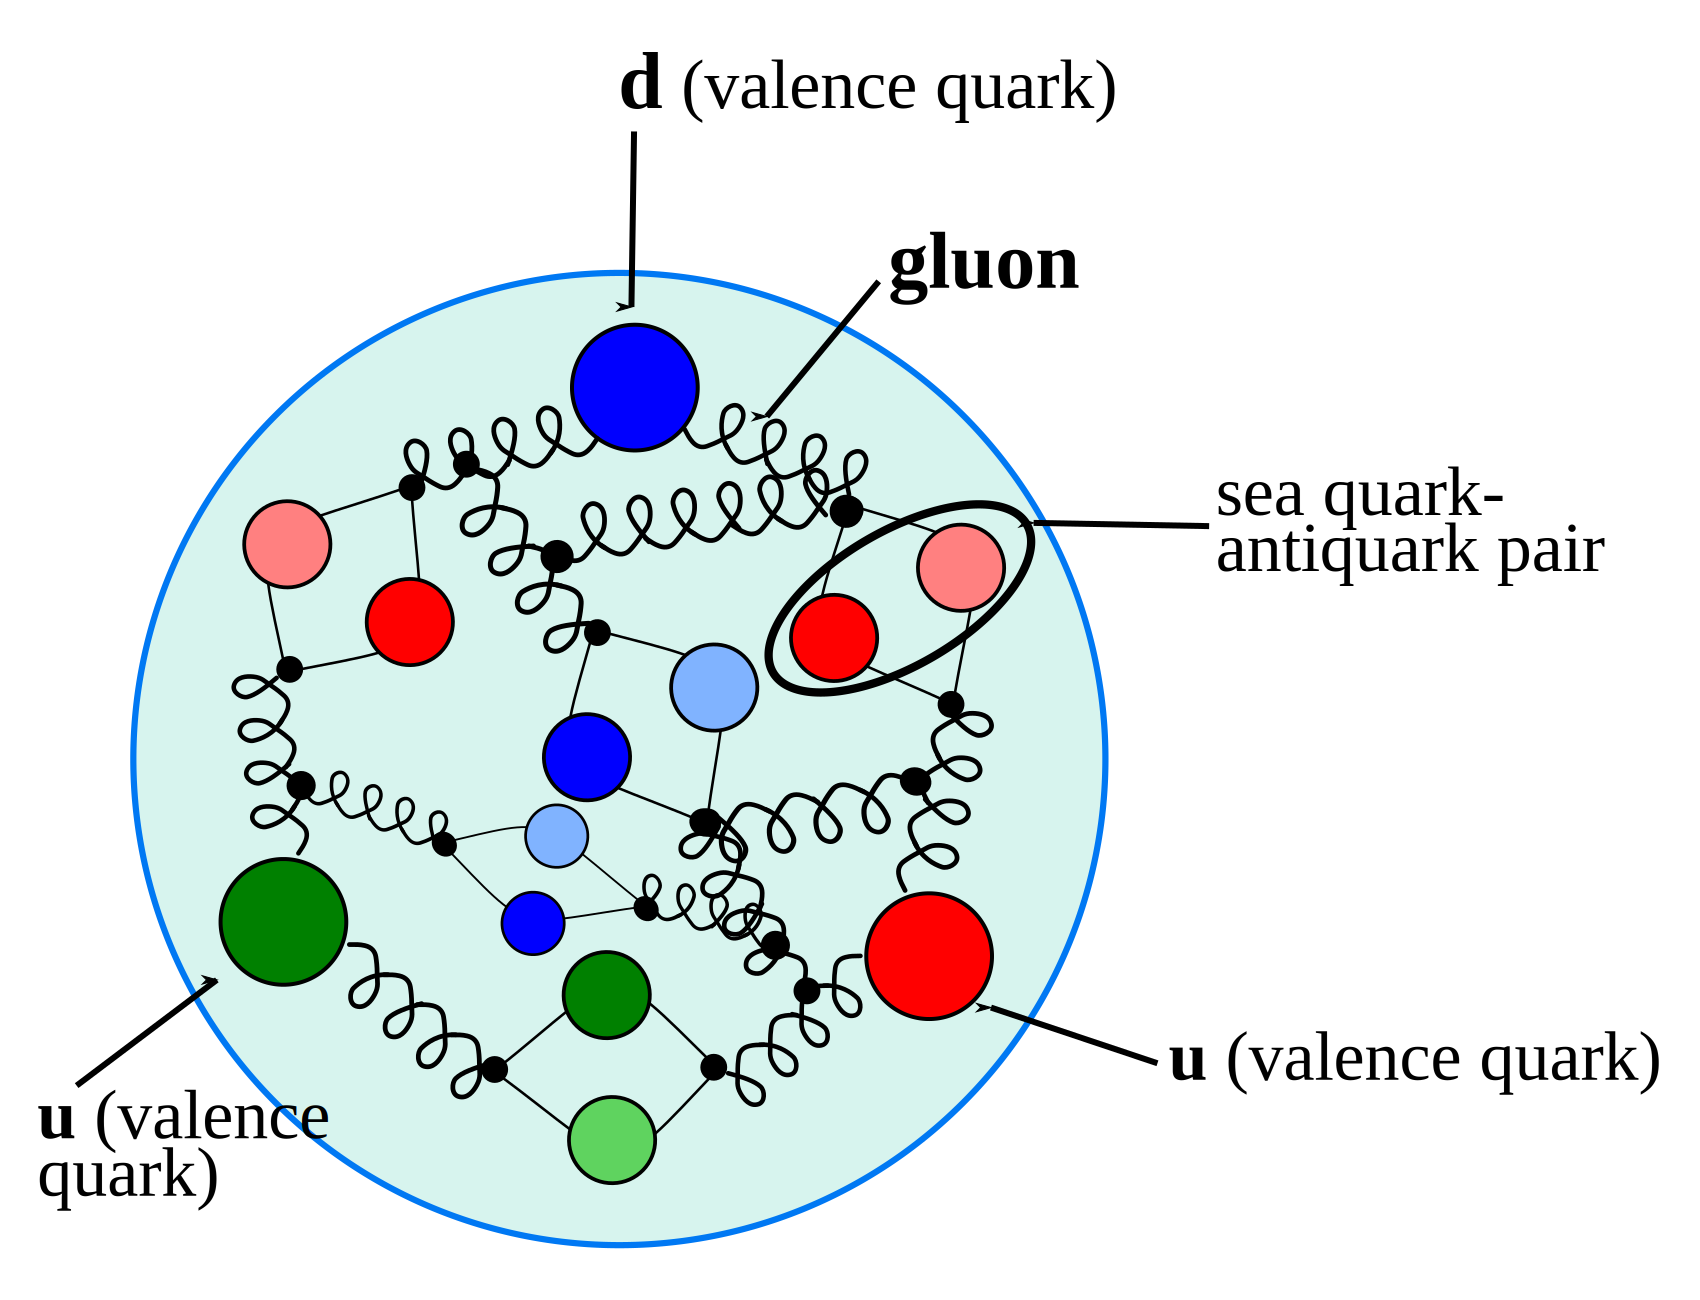
\includegraphics[width=0.45\textwidth]{../figs/Intro/protonStructure.png}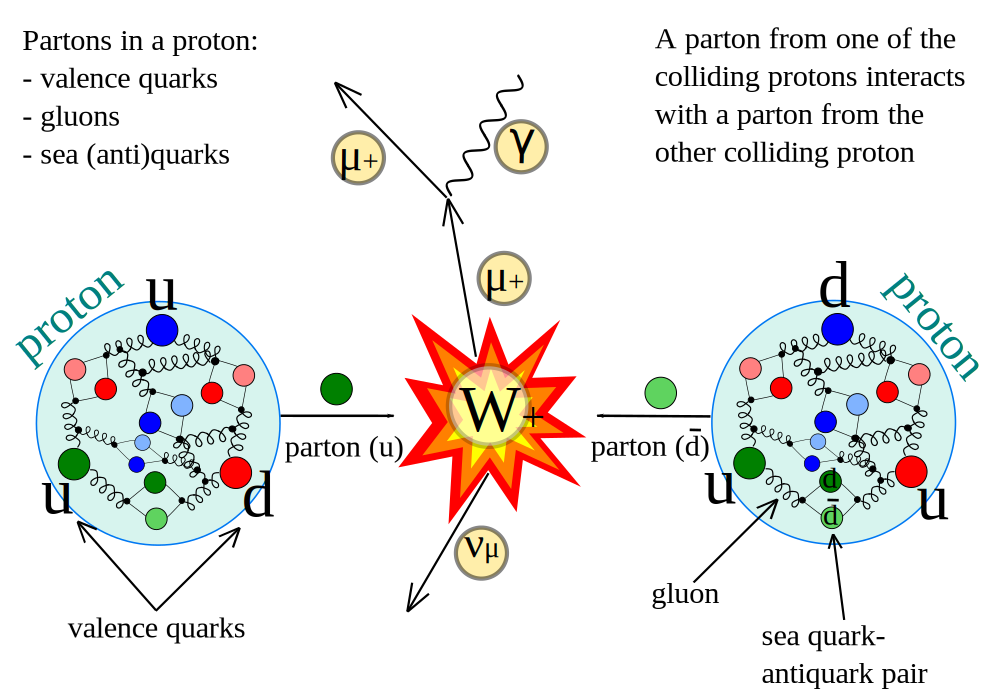
\includegraphics[width=0.45\textwidth]{../figs/Intro/ppCollision.png}}
    \caption{The proton structure (left) and the proton-proton collision (right).}
    \label{fig:ppCollision}
  \end{center}
\end{figure}

\begin{figure}[htb]
  \begin{center}
    {\includegraphics[width=0.85\textwidth]{../figs/Intro/pdfs.png}}
    \caption{Martin-Stirling-Thorne-Watt Parton Distribution Functions \cite{ref_fig_pdfs}}
    \label{fig:pdfs}
  \end{center}
\end{figure}


% ADD FIGURE WITH PDFs LIKE IN THE PRESENTATION

